\section{Project Management}
\subsection{Methodology}
To effectively manage time within this project of large nature and short time frame, several project management methodologies and principals were implemented. In order to select the correct approach to incorporate project management into this project, methodologies were chosen based on the projects needs. Time within the project needed to be allocated towards both theoretical and technical research, to select the technologies to be used, models for evaluation and to learn how to use the technologies to implement them. As well as this, time should also be invested into the implementation and training of the models used in this evaluation, this will ensure fair and accurate results, and ample time to perform training. The selected methodology should also allow for flexibility, if issues arise or any risks identified occur, the project can remain on track.

A kanban style approach was the selected project management methodology that met the above needs. The kanban approach is an agile methodology which divides a project into work items, which are then represented on a kanban board, splitting the work items into three categories: to do, in progress and complete. This is used alongside its four agile inspired principles: visualise workflow, limit work in progress, focus on flow and continuous improvement. Using this approach means that project members are only ever focused on work in progress, meaning that items in the backlog, or to do section, can be re-prioritised and changed without impacting the project, allowing for continuous improvement of the product. Some benefits of kanban, as reported by \cite{ahmad2013kanban}, highlight a better understanding of the entire project process as the visualisation of work items give developers a clear understanding of the project's direction. Kanban's limitation of work in progress items also minimises lead time, with the likes of BBC Worldwide reducing time to delivery by 37\% \citep{senapathi2011factors}.

However, there are some drawbacks to the kanban method. Most drawbacks identified by \cite{ahmad2013kanban} relate to its difficulty of implementation into pre-existing work cultures and teams. Since this project has a singular developer, these are not applicable. One drawback that this project must be mindful of is introduced by the lack of timing attached to work items, meaning that if not monitored correctly, the project could fall behind schedule due to over focusing on one work item. In order to mitigate these risks, some guidelines from the waterfall methodology were implemented into the project, namely its sequential project structure principle. The reasoning behind this combined approach allows for the limited multitasking and flexibility that kanban introduces combined with the set time planning of waterfall. In the context of this project, it will allow flexibility and adaptability, if the project's priorities change following regular supervisor meetings, or if issues occur. It will also allow constant iteration and improvement of models being evaluated while not being overwhelmed by multitasking.

While abiding by the guiding principles mentioned above, the project will make use of a kanban board for all work items, alongside a waterfall style Gantt chart to pre-plan the entire project's timeline, seen in \autoref{fig:gantt-chart}.

\begin{figure}[H]
    \centering
    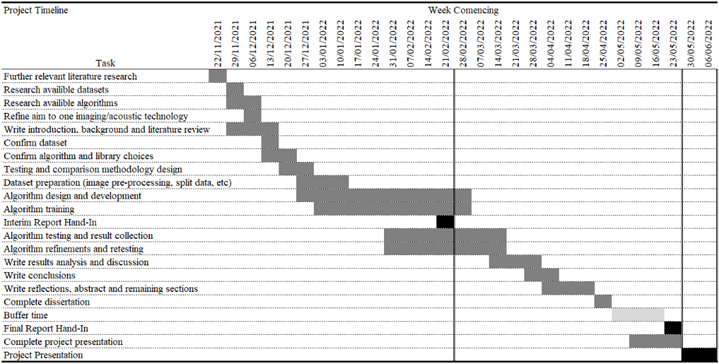
\includegraphics[width=\textwidth]{figures/gantt-chart.png}
    \caption{Project plan presented as a Gantt chart.}
    \label{fig:gantt-chart}
\end{figure}

\subsection{Risks} \label{risks}
During any project there are always risks that can be encountered and if no mitigation plan is in place, then it can lead to delays in the project. As part of the project management within this project, a full risk assessment was performed and mitigation planned to avoid any lost time. This was integrated into the project management methodology, by allowing for a buffer time within the waterfall plan of the overall project. The risk management table can be seen in \autoref{tbl:risk-table}.

\begin{table}[H]
    \caption{Risks likely to be encountered during this project.}
    \centering
    \begin{tabular}{p{0.22\textwidth}|p{0.11\textwidth}|p{0.14\textwidth}|p{0.41\textwidth}}
    Risk & Impact & Likelihood & Mitigation\\
    \hline\hline
    No availability of suitable training datasets. & High & Medium & While researching which imaging/sound source to use (CT, X-Ray, Acoustic), ensure there is sufficient availability of datasets and dataset size before beginning algorithm development.\\
    Algorithm requires significant computational performance that cannot be supplied. & Medium & Medium & When researching and selecting which machine learning algorithms will be used for evaluation, take note, and ensure that only resource efficient models are used. This will both mitigate the risk for training and testing the algorithms during this project and reflect hardware requirements of real-world use.\\
    Algorithm will not function due to   unavailable libraries or hardware requirements. & Medium & High & When selecting which machine learning algorithms will be used for evaluation, check each algorithm’s prerequisite hardware requirements, and ensure they are open source and available for use by all.\\
    Machine learning techniques or algorithms suddenly becomes closed source and cannot be used. & Medium & Low & Regularly check usage rights of each algorithm and select algorithms open source by nature.\\ 
    \end{tabular}
    \label{tbl:risk-table}
\end{table}

\section{Software Development}
Software development and the Software Development Life Cycle (SDLC) are important to all software products, solutions and research. The SDLC acts as a guide for the planning, development and delivery of any software focused project, in this case the planning of the problem domain, the development of multiple machine learning models and the delivery of evaluated results as a product of this software.

The kanban approach was again used to guide software development, taking the kanban board and sectioning work items into stages of the SDLC: Backlog, Requirements, Design, Development, Testing, Deployment, Done. Put into context, a model not yet developed or researched, would be placed into the backlog, moving into the requirements section as research into existing implementations and dependencies of the model were carried out. When a model was in the design section, the structure of the model (e.g. hidden layer formatting) was put in place. In development the model would be built within a development environment, tested in the testing section and finally evaluated against the dataset when in the deployment section. Once the evaluation is finished, it can then be placed in the done section.

Using this methodology when developing software for this project comes with the same advantages as it does for managing the project. Minimising work in progress means there is a focus on delivering working and evaluated models, while continually measuring and improving the life cycle of development for each model. This continual adaptability and flexibility means that kanban is especially suited to this project and serves the test and improve nature of it.

\section{Toolsets and Machine Environments}
There are a number of toolsets used within this project's artefact, both project management, software and hardware related. This section discusses and justifies the toolsets and machine environments used in this study.

\subsection{Project Management Software}
In order to facilitate the kanban style management of the project, there are several different solutions that could be used. Popular kanban board tools include Trello \citep{Trello41:online}, monday.com \citep{mondayco9:online} and GitHub Project Boards \citep{Aboutpro84:online}. While all share the same basic feature sets, for example, customising board sections and categorisation of work items, simplicity is a key requirement for a solo study such as this one. Trello boasts the simplest set up and usage of all three tools, with an easy and instant set up, and on-the-go customisation. Trello was the selected tool for the kanban board management of the SDLC, a snapshot of which can be seen in \autoref{fig:trello}.

\begin{figure}[H]
    \centering
    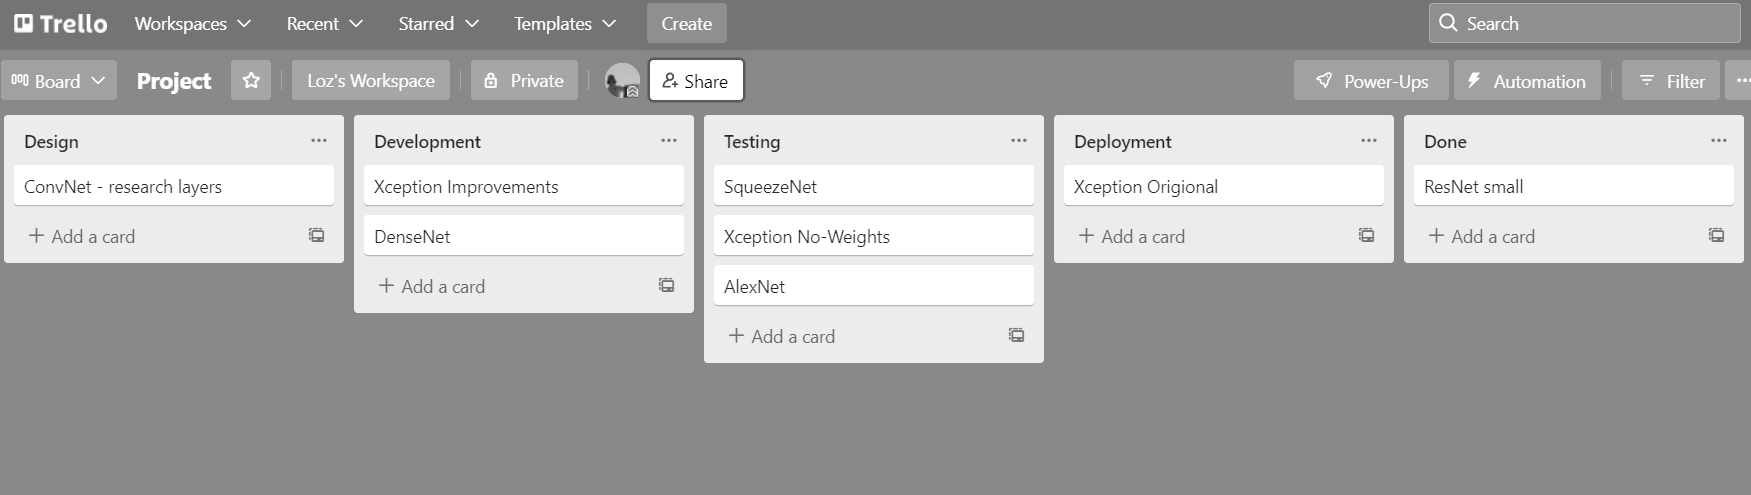
\includegraphics[width=\textwidth]{figures/trello.png}
    \caption{SDLC within Trello.}
    \label{fig:trello}
\end{figure}

\subsection{Software Toolsets and Development Environments}
The following sections introduce the software and development environments used to complete this research project.

\phantomsection
\subsubsection{Python}
Python was the chosen language for this project for a number of reasons. Firstly, Python is the most popular programming language worldwide, with a 27.85 \% market share, according to the PYPL index \citep{PYPLPopu3:online}, seen in \autoref{tbl:PYPL-table}. This means not only is it well known by computer and data scientists, it is also well supported by both its richness of available libraries and its documentation. Its popularity directly influences its choice for the project, by allowing others to pick up and further improve on findings from this research. 

\begin{table}[H]
    \caption{PYPL Worldwide Index, May 2022 \citep{PYPLPopu3:online}.}
    \centering
    \begin{tabular}{c|l|r}
        Rank & Language & Share \\
        \hline\hline
        1 & Python & 27.85\% \\
        2 & Java & 17.86\% \\
        3 & JavaScript & 9.17\% \\
        4 & C\# & 7.62\% \\
        5 & C/C++ & 7.0\% \\
        6 & PHP & 5.36\% \\
        7 & R & 4.34\% \\
        8 & TypeScript & 2.39\% \\
        9 & Objective-C & 2.25\% \\
        10 & Swift & 2.05\% \\
    \end{tabular}
    \label{tbl:PYPL-table}
\end{table}

Other languages in the PYPL list, such as Java, JavaScript and C\# also have a large community and wide documentation, however there are still other factors that set Python apart from these, making it the final choice. Python’s availability of libraries was also an important factor in its selection as most machine learning and deep learning libraries are supported by Python (e.g. TensorFlow, PyTorch and Scikit-Learn) and its dominance is expected to remain for the foreseeable future \citep{raschka2020machine}. This is compared to libraries like DeepLearning4j, a deep learning library for Java, which, while comparable to the Python libraries, has a declining use within the medical field \citep{erickson2017toolkits}. 

Finally, Python’s syntax, which is very close to the English language, makes it very readable, even by those with no prior knowledge of the language, unlike Java and C\# \citep{srinath2017python}.

\subsubsection{TensorFlow - Keras}
TensorFlow with Keras as the API layer was the chosen machine learning library for this project. TensorFlow is an "end-to-end open source platform for machine learning" with an eager execution environment \citep{TensorFl5:online}. TensorFlow is built upon tensors, which are immutable, multi-dimensional arrays, that are used to store objects, classes and weights that propagate through neural networks. TensorFlow was chosen over other libraries, such as PyTorch and Scikit-Learn, for several reasons.  Firstly, its eager execution means one can view results of operations instantly, as tensors are updated as they are called upon within the code. This allows one to quickly judge the success of a particular model instantly, as it trains, resulting in quick debugging. Another reason for choosing TensorFlow was its integration with Keras, an API written to run on top of TensorFlow, which makes the creation of machine learning models simple and fast with its sequential model \citep{AboutKer65:online}. The sequential model is a linear stack of layers which allows a user to prototype and build models from scratch or improve on an existing library of models easily. Keras supplies over 30 pre-trained deep learning models for use within its API, this is a key feature in this project as it allows for accurate replication of the chosen models for evaluation and use of transfer learning in selected models.

TensorFlow and Keras are amongst the most popular machine learning libraries for research studies and business use cases. They have a competitive edge in development support, which makes them both highly applicable in real world projects. \cite{hale2018deep} ranked each library against each other based on a power score, calculated by the weighted scores of popularities from multiple data sources, seen in \autoref{fig:ml-power-scores}. 

\begin{figure}[H]
    \centering
    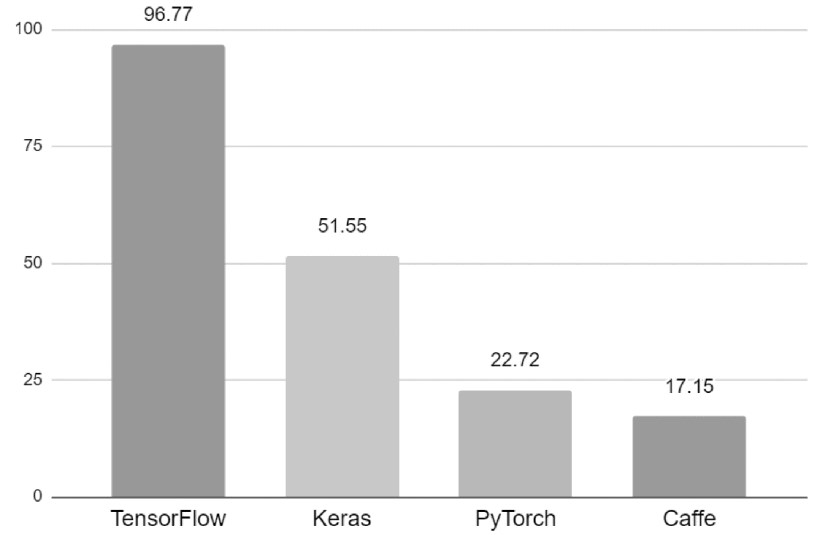
\includegraphics[width=0.65\textwidth]{figures/ml-power-sources.jpg}
    \caption{Power scores of various machine learning libraries \citep{hale2018deep}.}
    \label{fig:ml-power-scores}
\end{figure}

\subsubsection{TensorBoard}
TensorBoard is a visualisation library for TensorFlow, that tracks and plots metrics from TensorFlow models as they train \citep{TensorBo28:online}. Within this project, TensorBoard was used to extract visual data of the models performance, like accuracy and loss metrics, as well as tracking whether a particular model was over/under fitting. TensorBoard was chosen over other visualisation libraries, like Matplotlib or seaborn, due to its tight integration with TensorFlow, and interactivity. TensorBoard also allows one to implement and track hyper-parameter tuning within a project. This was extremely beneficial for this project, as it will allow for the best model selection from each class of models possible

\subsubsection{Scikit-Learn}
Scikit-Learn is a machine learning library built for Python, which is bundled with many evaluation functions \citep{33Metric9:online} and cross validation functions \citep{31Crossv34:online}. The evaluation functions used within Scikit-Learn provided accuracy, precision, recall, F1 score and confusion matrix metrics, for each trained model in the project. Scikit-Learn's evaluation functions were chosen over Keras' inbuilt functions as Keras' own evaluation functions are limited to only providing loss and accuracy data \citep{Modeltra48:online}, with other metrics having to be calculated manually, making Scikit-Learn a faster and easier to implement solution. 

Scikit-Learn's Stratified K-Fold \citep{sklearnm1:online} cross validation implementation was also used within this project. It was used to ensure fairness when evaluating the performance of the models, by taking an average of each fold's validation accuracy the possibility of dataset or training inconsistencies are removed. Keras offers no in-built solution to cross validation, so much like the evaluation metrics, it has to be performed manually, making Scikit-Learn a faster and easier solution to implement.

Scikit-Learn was also used to shuffle and re-sample the training data, so that there was no bias towards a particular class or model due to possible bias in the dataset structure.

\subsubsection{Pandas}
Pandas is an open-source data manipulation and analysis library for Python \citep{pandasPy63:online}. For this project, pandas was valuable in carrying out initial pre-processing when loading in the dataset to the artefact, for example, dropping patient data from the dataset to remove bloat. In addition, pandas DataFrames were used to store and handle the dataset throughout the artefact; this is a two-dimensional structure designed to store tabular data such as dataset labels.

\subsubsection{NumPy}
NumPy is an open-source scientific and mathematics library for Python \citep{NumPy90:online}. NumPy was used for basic numerical operations within the project and was also a dependency for other libraries used.

\subsubsection{Google Cloud Platform - Development Environment}
Google Cloud Platform was used in this project to train and test the initial selection of the six COVID-19 classification models and perform hyper-parameter tuning on each model. Two services used within Google Cloud Platform were Vertex AI \citep{VertexAI57:online} and Cloud Storage \citep{CloudSto72:online}. Vertex AI enables fast code building though Vertex AI Workbench, a Jupyter notebook environment with access to server grade GPUs. This enabled quick testing and finalisation of the first round of models for evaluation within this project. Vertex AI also has the ability to execute notebook runs on specific hardware and software instances in parallel, meaning fairness though out the first stages of model evaluation and a fast training time due to the allocated NVIDIA Tesla K80s for each instance. Cloud storage was used to store the COVIDx-CXR database the models were trained on, alongside the saved trained model weights and the TensorBoard logs.

\subsubsection{Google Colab - Development Environment}
Google Colaboratory (Colab) is an online Jupyter notebook style Python development environment designed for machine learning and data analysis \citep{GoogleCo52:online}. Colab is equipped with pre-installed data manipulation and machine learning libraries, including all those used in this project, and provides access to fast computing resources like GPUs. This makes developing and executing machine learning experiments, like this project, accessible and fast, with the ability to share with other researchers. This development environment was used for the initial building of all models, and the final evaluation of the best models found. One downside, however, is the fact that computing resources are not guaranteed, meaning that if demand for resources is high, or a notebook has been running for particularly long, then there is a possibility that it might be terminated.

\subsubsection{GitHub}
GitHub is an online Git version control software offering source code management and internet hosting for projects. In this project GitHub was used as both a version control software and a code hosting tool, to ensure there was a backup of all code, for each version authored, and for seamless transfers between Google Cloud Platform and Google Colab.

\section{Research Methods}
Different research methods were used in this project to gather and analyse the data collected, and to evaluate the selected models'. This project takes an inductive approach towards the research process, by making observations and recording results of models performance and proposing theories and explanations for why particular models may perform better from the collected data \citep{saunders2009research}. The analysis of data collected in this project is quantitative, the full list of which is detailed later in this section. Using quantitative analysis allows for statistical analysis of results such that decisions and recommendations can be verified and evaluated by the data collected \citep{saunders2009research}. The majority of this study makes use of primary data collected, as the main strategy of data collection is the experiment (training and analysing the models) \citep{hox2005data}. However to position the results amongst other studies and justify findings, some comparisons will be drawn between other studies identified in the literature review, using secondary data. Primary data collected should take a ratio form that can be ranked with set intervals, for example, a percent between accuracy score and a true zero point (e.g. a 0 accuracy score means an absolute lack in classification ability). Results will be represented in a combination of graphical and tabular form, depending on the metric and ease of comparability. 

Once the research methodology of a project has been defined, it is important to consider the strategy for collecting and formatting the qualitative primary data. The following sections detail how the research was carried out and the particular testing structures that were set in place.

\subsection{Dataset Organisation}
The COVIDx-CXR dataset selected for use, discussed in the literature review, contains 30,482 X-Ray images, with the binary classification labels' containing 13,992 negative cases and 16,490 positive cases. This slight skew in the labels proportions means that it has the potential to introduce some bias in training. To mitigate this, the dataset should be balanced using a down sampling method before training. When performing multi-label classification on the dataset, the split of 8,085 normal, 5,555 pneumonia and 16,490 COVID-19 cases, should also be balanced using the same method.

The images within the dataset are also of varying sizes and colour spaces. This could lead to further skewing of results in training, and if the images are particularly large, much slower training times. To combat this, all images should go through a pre-processing stage before being passed to a model for training. Pre-processing should down-sample all images to a smaller and equal resolution, an equal colour space, as well as performing random transformations to the image. These transformations, like flipping, rotating and cropping, should mitigate any model bias towards images sharing the same orientation, so in practice an X-Ray image to be evaluated by the model will not be treated differently if its orientation or cropping is not the same as the datasets.

Since the dataset is so large, it would not be feasible to train all models and hyper-parameter variations on the entire dataset. The database was reduced to a smaller size for the initial training and model improvement rounds, discussed below. The small size of the dataset was to be 1,500 images, 750 negative cases, 750 positive cases in the case of binary classification, or 500 normal, 500 pneumonia and 500 COVID-19 cases in the case of multi-label classification.

To ensure further fairness in model testing, a cross validation method, stratified K fold, was used in the models training. Stratified K fold splits the dataset into a defined number of groups and for each fold (iteration) one of those groups is chosen as a validation (test) dataset, while the rest is used as training data. This new group is chosen for each iteration, until each group has been used as a test dataset. To ensure fairness, stratified K fold also splits the data in a way so that each group contains the same number of images of each class. The results from each fold are then averaged together to produce the validation results from training. This entire process ensures the entire dataset is tested, while also accounting for the minor changes in results from each model when trained.

\subsection{Model Training and Data Collection} \label{model-training}
Firstly, the structure to gather the primary quantitative data was devised, this ensured an unbiased and fair standard was followed for each model. The structure is detailed throughout the following sections.

\phantomsection

\subsubsection{Initial Training}
All six models were optimised using hyper-parameter tuning using a Google Cloud Platform Vertex AI parallel notebook execution process. This was performed on a small portion of the COVIDx-CXR dataset, meaning the training time for larger models did not exceed the allotted time for this stage of the project and allotted hardware resources within Google Cloud Platform were not depleted. All models were trained with the same batch size of 32, the same image resolution of 224 x 224 pixels, the same maximum allowed epochs (20) and the same number of stratified K folds (5) for cross validation.

Once each model with each variation of hyper-parameters had been trained, each fold of each model was evaluated on the test dataset (a separate 400 chest X-Ray images). Once the evaluation was performed, the average metrics from the test dataset across the 5 folds of each model were calculated. These metrics would then be used to select the best performing model, with the best hyper-parameters.

\subsubsection{Model Improvements}
The best performing model and hyper-parameters then went under a trial and error improvements round. The models were tested using model improvements and network formats, as sourced in the literature review and in further research. For each attempted improvement the model was evaluated in the same manner as the initial training, this was replicated for several rounds until improvements produced diminishing returns. Once the evaluation was performed on each round of improvements, the average metrics from the test dataset across the 5 folds of each model were calculated. These metrics were then used to select the best performing model improvements.

\subsubsection{Final Training}
Finally the best performing model, hyper-parameters and improvements were trained on both a small portion of the database and the entire database. Detailed metrics of accuracy across each fold for both the validation and test data were recorded. In order to measure the success of the improvements, two additional models of the same architecture were trained on both a small portion of the database and the entire database. These models have no improvements and no pre-trained weights (if applicable for the winning model) respectively.

\subsubsection{Multi-Label Training}
The best model, hyper-parameters and improvements, as well as the base model with no improvements were trained on both a small portion of the multi-label database and the entire multi-label database. Detailed metrics of accuracy across each fold for both the validation and test data were recorded. These metrics were then used to compare the models developed in this study to other similar studies identified in the literature review. This helped to gauge how well the models performed relative to other studies.

\subsection{Metrics}
In order to measure the performance of the models and their various iterations, several performance metrics were recorded. The following is a list of metrics and their definitions. Note that $TP$ is equal to true positives, $TN$ is equal to true negatives, $FP$ is equal to false positives and $FN$ is equal to false negatives.

The first performance metric was accuracy. To measure this, the fraction of correct predictions over the total number of samples was used to distinguish each model and variations performance. In this case, the best value is 1 and the worst is 0. The definition of accuracy can be seen in \autoref{eq:accuracy}.

\begin{align}
\text{accuracy}= \frac{TP+TN}{TP+TN+FP+FN}
\label{eq:accuracy}
\end{align}

Secondly, precision, measures the models' ability not to classify a negative sample as positive, and is used to measure the likelihood a model will return a false positive. In this case, the best value is 1 and the worst is 0. The definition of precision can be seen in \autoref{eq:precision}.

\begin{align}
\text{precision}= \frac{TP}{TP+FP}
\label{eq:precision}
\end{align}

Thirdly, recall, measures the ability of a model to correctly classify, or find, all the positive samples, where the best value is 1 and the worst is 0. The definition of recall can be seen in \autoref{eq:recall}.

\begin{align}
\text{recall}= \frac{TP}{TP+FN}
\label{eq:recall}
\end{align}

Fourth, F1 score, is the harmonic mean of the precision and recall. This shows the accuracy of models’ positive predictions. In this case, the best value is 1 and the worst is 0. The definition of F1 score can be seen in \autoref{eq:f1-score}.

\begin{align}
\text{F1 score}= 2 \times \frac{precision \times recall}{precision + recall}
\label{eq:f1-score}
\end{align}

The fifth metric recorded was the confusion matrix, which is a table classifying all the predictions of the model into the respective $TP$, $TN$, $FP$ and $FN$ values. An example can be seen in \autoref{tbl:confusion-matrix-table}.

\begin{table}[H]
    \caption{A confusion matrix.}
    \centering
    \begin{tabular}{cccc}
     &  & \multicolumn{2}{c}{True Class} \\ \cline{3-4} 
     & \multicolumn{1}{c|}{} & \multicolumn{1}{c|}{Positive} & \multicolumn{1}{c|}{Negative} \\ \cline{2-4} 
    \multicolumn{1}{c|}{\multirow{2}{*}{\rotatebox[origin=c]{90}{\makecell{Predicted \\ Class}}}} & \multicolumn{1}{c|}{Positive} & \multicolumn{1}{c|}{TP} & \multicolumn{1}{c|}{FP} \\ \cline{2-4} 
    \multicolumn{1}{c|}{} & \multicolumn{1}{c|}{Negative} & \multicolumn{1}{c|}{FN} & \multicolumn{1}{c|}{TP} \\ \cline{2-4} 
    \end{tabular}
    \label{tbl:confusion-matrix-table}
\end{table}

Finally the training time and number of trainable parameters for each model was recorded. This was classified as the time a model took to train on test data and perform validation after each epoch, and did not include test evaluation time. This shows both the models speed, but also size, with larger models taking longer to train.